\section{Semaine 15 : 15/05/2023 - 19/05/2023}
\graphicspath{{semaines/semaine_15/images/}}

\setcounter{equation}{0}

\begin{abstract}
	(Killian est en vacances pour les deux prochaines semaines)
	
	Au tout début de la semaine, j'ai fait un petit test où je comparais la méthode duale pour le rehaussement en prenant comme fonction test $v$ ou $\tilde{\phi}v$. On s'est rendu compte que cela nous donnait les mêmes résultats.
	
	Comme Emmanuel était de retour cette semaine, on a fait une réunion mardi avec Michel. Après avoir montré mes résultats sur le FNO, on a cherché des solutions afin de comprendre pourquoi ces résultats sont très différents des résultats obtenus sur la solution analytique. Dans un premier temps, ils ont proposés de tester d'implémenter un réseau multiperceptron qui nous permet d'obtenir une solution en tout point de notre domaine et donc de pouvoir tester la correction avec $\tilde{\phi}$ de de plus haut degré (10 par exemple). Par la suite, ils ont proposés une seconde idée, plus simple, qui consiste à construire une solution analytique à partir de la sortie du FNO. Ils ont proposés de tester avec Fourier, Legendre ou Hermite. J'ai alors commencé à tester avec Fourier cette semaine, les explications et résultats seront mis dans le suivi de la semaine suivante. 
	
	De plus, j'ai repris les explications de Michel sur la preuve de l'inégalité obtenu pour le rehaussement et ait rédigé un petit document qui n'est pas encore terminé. Je vais mettre ce document ici.  
\end{abstract}

\subsection{Comparaison fonction test - Rehaussement}

Résultats obtenus :

\begin{minipage}{\linewidth}
	\centering
	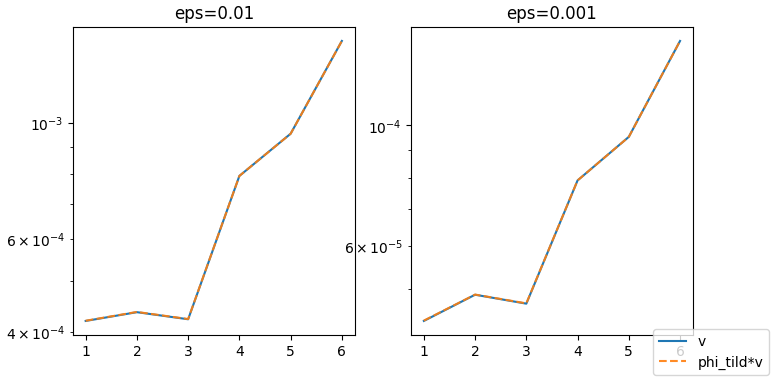
\includegraphics[width=0.4\linewidth]{test_fct_test.png}
\end{minipage}

\subsection{Estimation d'erreur - Problème rehaussé (Modifié!) \faBookmarkO}

On se place ici dans le cadre de FEM standard. 

\textbf{Problème initital :} \\
On considère initialement le problème de Poisson avec condition de Dirichlet homogène ou non homogène :
\begin{equation}
	\left\{\begin{aligned}
		&-\Delta u=f \quad &&\text{dans } \Omega \\
		&u=g \quad &&\text{sur } \Gamma
	\end{aligned}\right. \label{pb_initial} \tag{$\mathcal{P}$}
\end{equation}

\textbf{Problème considéré :} \\
Dans notre cas, on souhaite appliquer une correction à la sortie d'un FNO.
On va considérer ici que l'on possède une solution analytique $u_{ex}$ et qu'après une utilisation du FNO, on obtient une solution du type
$$\tilde{\phi}(x,y) = u_{ex}(x,y)-\epsilon P(x,y)$$
avec $P$ la perturbation (tel que $P=0$ sur $\Gamma$) et $\epsilon$ petit.

On considère
$$\hat{\phi}=\tilde{\phi}+m=u_{ex}-\epsilon P+m=\widehat{u_{ex}}-\epsilon P$$
avec $\widehat{u_{ex}}=u_{ex}+m$ et $m$ une constante.

On souhaite alors résoudre le problème suivant :
\begin{equation}
	\left\{\begin{aligned}
		&-\Delta (\hat{\phi}C)=f \quad &&\Omega \\
		&(\hat{\phi}C)=g+m \quad &&\Gamma
	\end{aligned}\right. \label{pb_reh} \tag{$\mathcal{C}$}
\end{equation}

On pose alors
$$\hat{u}=\hat{\phi}C$$

\textbf{But du document :} \\
Démonter la propriété suivante :
\begin{equation}
	\left|\left|\hat{u}-\hat{u_h}\right|\right|_0\le ch^{k+1}||\hat{\phi}||_\infty\left|C\right|_{k+1}
	\label{ine_a_dem}
\end{equation}

\textbf{Problèmes variationnels :} \\

Problème variationnel :
$$\text{Trouver } \hat{u}\in V \text{ tel que } a(\hat{u},v)=l(v), \;\forall v\in V$$

Problème variationnel approché :
$$\text{Trouver } \hat{u_h}\in V_h \text{ tel que } a(\hat{u_h},v_h)=l(v_h), \;\forall v_h\in V_h$$

\subsubsection{Partie 1 : norme $H^1$}

Comme $V_h$ est un sous espace vectoriel de $V$, en posant $v=v_h$, on obtient :
$$a(\hat{\phi}C,\hat{\phi}v_h)-a(\hat{\phi}C_h,\hat{\phi}v_h)=0 \quad \forall v_h\in V_h$$
On a alors l'orthogonalité de Galerkin : \color{red}{(ATTENTION : Abus de notation sur $v_h$ !)}\color{black}
$$a(\hat{u}-\hat{u_h},v_h)=0 \quad \forall v_h\in V_h$$
On a alors
\begin{align*}
	\color{red}{\nu}\color{black}||\hat{u}-\hat{u_h}||_1^2&\le\alpha a(\hat{u}-\hat{u_h},\hat{u}-\hat{u_h}) &&\text{par coercivité} \\
	&=\alpha a(\hat{u}-\hat{u_h},\hat{u}-I_h\hat{u}+I_h\hat{u}-\hat{u_h}) \\
	&=\alpha a(\hat{u}-\hat{u_h},\hat{u}-I_h\hat{u}) &&\text{par orthogonalité de Galerkin en prenant } v_h=\hat{u_h}-I_h\hat{u} \\
	&\le\alpha |\hat{u}-\hat{u_h}|_1|\hat{u}-I_h\hat{u}|_1 &&\text{par continuité} \\
	&\le\alpha ||\hat{u}-\hat{u_h}||_1|\hat{u}-I_h\hat{u}|_1
\end{align*}
Ainsi
$$||\hat{u}-\hat{u_h}||_1\le\alpha|\hat{u}-I_h\hat{u}|_1$$
Or 
$$|\hat{u}-I_h\hat{u}|_1=|(C-I_hC)\hat{\phi}|_1$$
En posant $A=C-I_hC$, on a
$$|A\hat{\phi}|_1=||(A\hat{\phi})'||_0=||A'\hat{\phi}+A\hat{\phi}'||_0\le||A'\hat{\phi}||_0+||A\hat{\phi}'||_0$$
Comme
$$||A'\hat{\phi}||_0=\sqrt{\int_\Omega(A'\hat{\phi})^2}\le \max_\Omega \hat{\phi}\sqrt{\int_\Omega(A')^2}=||\hat{\phi}||_\infty|A|_1\le||\hat{\phi}||_\infty||A||_1$$
et
$$||A\hat{\phi}'||_0=\sqrt{\int_\Omega(A\hat{\phi}')^2}\le \max_\Omega \hat{\phi}'\sqrt{\int_\Omega(A)^2}=||\hat{\phi}'||_\infty||A||_0\le \alpha||\hat{\phi}||_\infty||A||_1$$
Ainsi
$$|A\hat{\phi}|_1\le\alpha ||\hat{\phi}||_\infty||A||_1$$
Donc
$$|\hat{u}-I_h\hat{u}|_1=|(C-I_hC)\hat{\phi}|_1\le\alpha ||\hat{\phi}||_\infty||C-I_hC||_1$$

Finalement en utilisant l'inégalité d'interpolation, on obtient
\begin{equation}
	\boxed{||\hat{u}-\hat{u_h}||_1\le\alpha h^k ||\hat{\phi}||_\infty |C|_{k+1}}
	\label{norme_H1}
\end{equation} 

\subsubsection{Partie 2 : norme $L^2$}

On applique la méthode de dualité d'Aubin-Nitsche. On considère le problème dual : \\
Soit $\hat{z}\in H_0^1(\Omega)$ solution du problème
$$\left\{\begin{aligned}
	&-\Delta\hat{z}=\hat{e_h} \quad &&\text{dans }\Omega \\
	&\hat{z}=0 \quad &&\text{sur } \Gamma
\end{aligned}\right.$$
avec $\hat{e_h}=\hat{u}-\hat{u_h}$.
Alors
$$a(u,v)=-\int_\Omega\Delta u\cdot v=\int_\Omega\nabla u\cdot\nabla v$$
et comme $e_h\in H_0^1(\Omega)$
\begin{equation}
	a(\hat{z},\hat{e_h})=\int_\Omega(-\Delta \hat{z})\cdot \hat{e_h}=\int_\Omega \hat{e_h}^2=||\hat{e_h}||_0^2
	\label{norme_e_h}
\end{equation}
De plus, par les propriétés de régularité : 
\begin{equation}
	\hat{z}\in H^2(\Omega)
	\label{z_H_2}
\end{equation}
et
\begin{equation}
	||\hat{z}||_2\le \alpha||\hat{e_h}||_0 =\alpha||\hat{u}-\hat{u_h}||_0
	\label{prop_reg}
\end{equation}
Ainsi
\begin{align*}
	||\hat{u}-\hat{u_h}||_0^2&=||\hat{e_h}||_0^2 \\
	&=a(\hat{z},\hat{e_h}) &&\text{par \ref{norme_e_h}} \\
	&=a(\hat{z}-I_h\hat{z},\hat{e_h}) &&\text{par orthogonalité de Galerkin} \\
	&\le\alpha|\hat{z}-I_h\hat{z}|_1|\hat{e_h}|_1 &&\text{par continuité} \\
	&\le\alpha h|\hat{z}|_2|\hat{e_h}|_1 &&\text{par \ref{z_H_2} et par inégalité d'interpolation} \\
	&\le\alpha \cdot h|\hat{z}|_2 \cdot h^k||\hat{\phi}||_\infty |C|_{k+1} &&\text{par \ref{norme_H1}} \\
	&\le\alpha h^{k+1}||\hat{u}-\hat{u_h}||_0||\hat{\phi}||_\infty |C|_{k+1} &&\text{par \ref{prop_reg}}
\end{align*}
Finalement
\begin{equation}
	\boxed{||\hat{u}-\hat{u_h}||_0\le\alpha h^{k+1}||\hat{\phi}||_\infty |C|_{k+1}}
\end{equation}

\begin{Rem}
	On notera que
	$$||\hat{u}-\hat{u_h}||_0=||u+m-(u_h+m)||_0=||u-u_h||_0$$
\end{Rem}

\conclusion{Les tests effectués avec Fourier pour obtenir une solution analytique à partir de la solution produite par le FNO seront mis à la semaine prochaine.

Il faudra continuer la preuve commencé cette semaine mais ce n'est pas une priorité.

(Ce document a été modifié.)}